\section{Theoretical Analysis}
\label{sec:analysis}

In these section we represent the plots that were produced by our theoretical analysis. These plots represents the Voltage on Envelope Detector and the output voltage of the circuit.



\FloatBarrier
\begin{figure}
  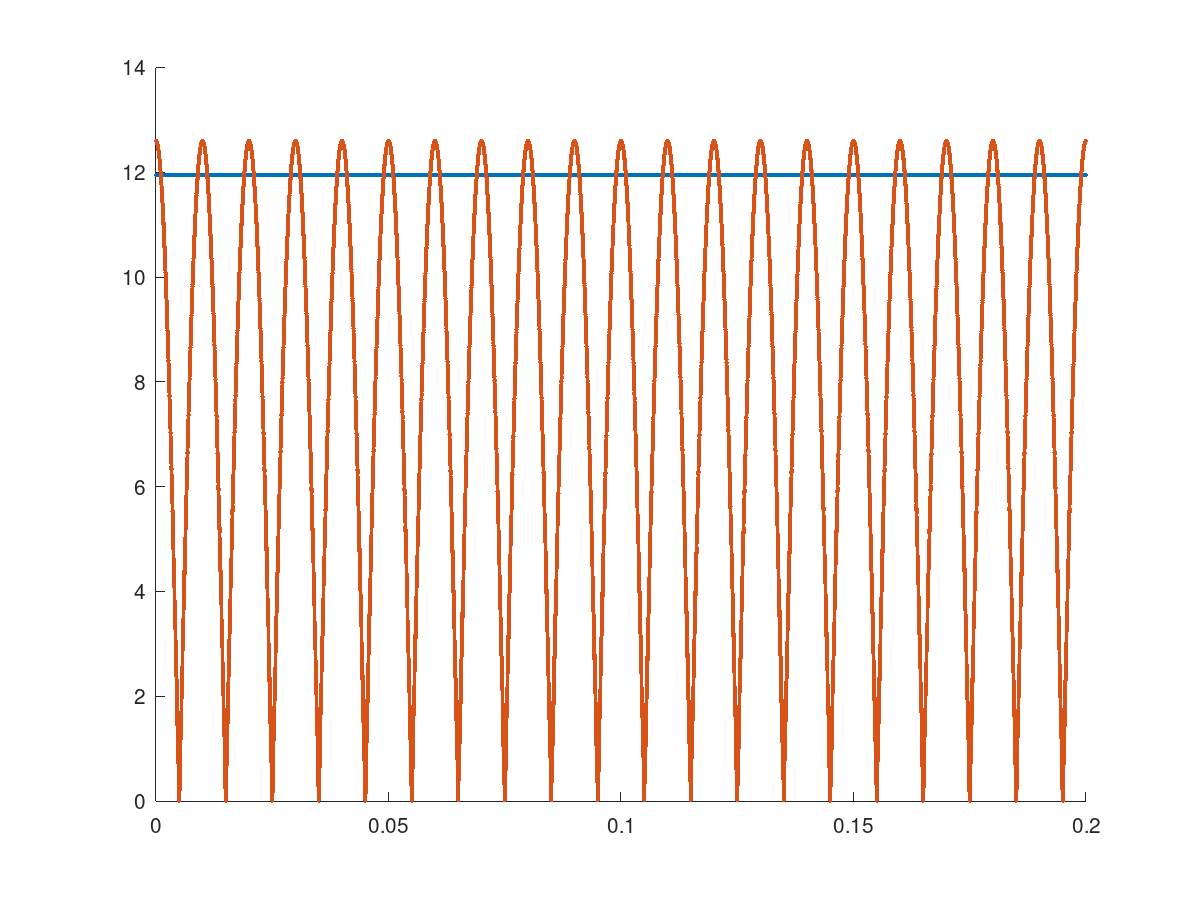
\includegraphics[width=\linewidth]{Condensador.png}
  \caption{Envelope Detector and Output Voltages}
  \label{fig:theoplots}
\end{figure}
\FloatBarrier

And finally to conclute the requirements for the theoretical analysis, we have computed the results of the voltage ripple and the output DC level.

\FloatBarrier
\begin{table}[h]
  \centering
  \begin{tabular}{|c|c|c|c|c|c|c|}
    \hline    
    
 $V_{ripple}$ & $V_{DC}$ \\ 
 2.61313e-05 V   & 11.95 V\\

    \hline
  \end{tabular}
  \caption{Ripple and DC voltages}
  \label{tab:Octave}
\end{table}
\FloatBarrier 






%\par The values of resistances R1 and R2 and capacitance C were chosen arbitarily in order to obtain the best possible results and also achieve the best merit, that is, the use of the minimum possible of each component. These values are shown down bellow: 

%colocar valores aqui 

%\par According to the conventional way, the transformers wires are coiled, so assuming that, in order to produce a downwards current through the Tranformer 1 and an upwards current through the Transformer 2, we have the correlation that:

%\begin{equation}
%  V_(t1)= n*V_(t2)
%  \label{}
%\end{equation}    

%where $n$ is the number of turns seen in Transformer 1; $V_(t1)$ is the AC signal in Transformer 1; V_(t2) is the signal in Transformer 2.  

%\par Because the objective is to obtained a DC voltage of 12V in the output, a sinusoidal signal of amplitude $qq coisa não esquecer$ was used for transformer number 2. 

%\par Due to (a certain number of diodes) in the full-wave bridge rectifier circuit, the voltage through resistance $R_1$ can be compute as: 

%\begin{equation}
 % V_(0_(rect))=|V_(t2)|
%  \label{}
%\end{equation}    

%For these theoretical analysis an ideal diode model has been considered and a capacitor, who is in charge to keep the volatge mainly constant and close to 12V. For that matters the time that it takes to the diode circuit to go OFF and for the capacitor to start discharging through the $R_1$ is given by: 

%\begin{equation}
%  V_(0_(rect))=|V_(t2)|
%  \label{}
%\end{equation}    
